\section{Methodology}
\label{sec:methods}

\subsection{Training and evaluation pipeline}
We train all classifiers from scratch using the shared data splits in
Section~\ref{sec:splits}. Each training batch passes through the model to produce
ten class scores, and we update the weights to minimize cross-entropy.
After each epoch, we evaluate validation loss with dropout disabled and batch
normalization using its running statistics. We use the checkpoint with the
lowest validation loss for testing. This allows the selected model to come
from an earlier epoch if validation performance deteriorates before training
ends. Every model still receives the same 50-epoch training budget.

\subsection{Model architectures}
\label{sec:architectures}
Each model maps an image to a feature vector $h\in\mathbb{R}^{d}$ and then
computes ten logits, $z=Wh+b$. The following descriptions use Fashion-MNIST
shapes. MNIST uses the same dimensions. CIFAR-10 has three-channel
$32\times32$ images. Table~\ref{tab:arch-comparison} summarizes feature
dimensions and parameter counts.

\subsubsection{Linear classifier}
The linear model flattens an image to $x\in\mathbb{R}^{784}$ and computes
$z=Wx+b$, where $W\in\mathbb{R}^{10\times784}$ and $b\in\mathbb{R}^{10}$.
Each class score is an affine function of the pixels. Flattening keeps the pixel
order. The model has no convolution or shared spatial filters and is our baseline. It tests how far class-specific weighted sums of pixels can go before adding
nonlinear layers or explicitly modelling spatial relationships.

\begin{figure}[htbp]
\centering
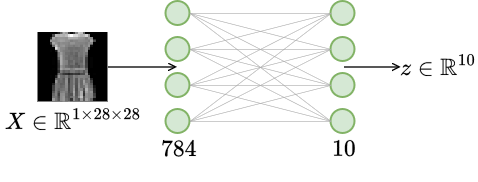
\includegraphics[width=0.75\linewidth]{Images/models/linear.png}
\caption{Linear classifier. The flattened image is mapped to ten class logits.}
\label{fig:model-linear}
\end{figure}

\subsubsection{Multilayer perceptron}
The MLP applies two hidden affine layers of widths 256 and 128 to the flattened
image. Each hidden layer is followed by ReLU and dropout with probability
$0.2$. A linear head maps the 128-dimensional features to ten logits. The
MLP learns nonlinear combinations of pixels but does not share weights across
image positions. Comparing it with Linear tests whether nonlinear pixel
combinations improve classification, while its comparison with CNN also
introduces local connectivity and shared filters.

\begin{figure}[htbp]
\centering
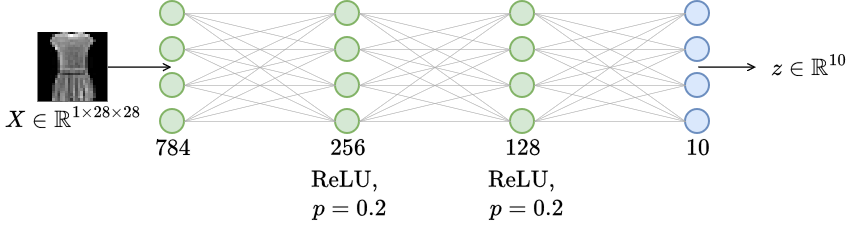
\includegraphics[width=0.95\linewidth]{Images/models/mlp.png}
\caption{MLP with hidden widths 256 and 128, ReLU, and dropout.}
\label{fig:model-mlp}
\end{figure}

\subsubsection{Convolutional neural network}
The CNN applies two convolutional blocks with 32 and 64 channels. Each
block contains a $3\times3$ convolution with stride 1 and padding 1, batch
normalization, ReLU, and $2\times2$ max pooling with stride 2. Convolution
biases are disabled. For a $28\times28$ image, the blocks produce
$32\times14\times14$ and $64\times7\times7$ feature maps. Flattening gives
3,136 values, followed by a 128-unit linear layer and ReLU. A ten-class
linear head produces the logits. For CIFAR-10, the final feature map is
$64\times8\times8$, so the hidden layer receives 4,096 values.

Convolution shares local filters across image positions. Flattening preserves
the positions of their responses, and the hidden layer can combine responses
across the full feature map. The classifier has 421,738 parameters for grayscale
images and 545,194 for CIFAR-10.

\begin{figure}[htbp]
\centering
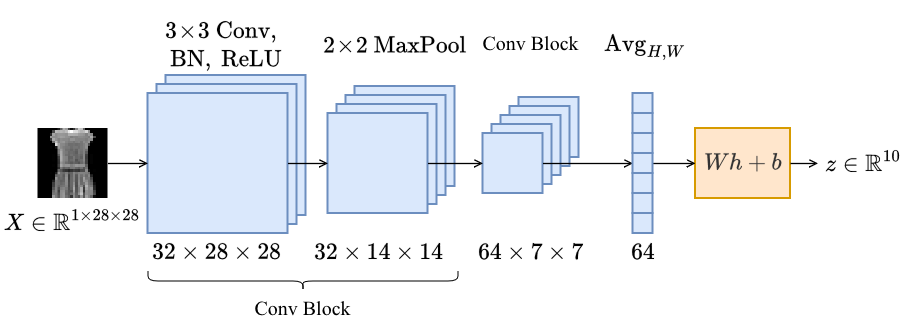
\includegraphics[width=0.95\linewidth]{Images/models/cnn.png}
\caption{CNN for MNIST and Fashion-MNIST. Flattened convolutional features feed a 128-unit hidden layer and the classification head.}
\label{fig:model-cnn}
\end{figure}

\subsubsection{Gated recurrent unit}
The GRU reads the image rows from top to bottom. An input of shape
$C\times H\times W$ becomes a sequence of $H$ vectors in
$\mathbb{R}^{CW}$. Fashion-MNIST gives 28 steps with 28 values per step.
CIFAR-10 gives 32 steps with 96 values per step.

The model has one recurrent layer with hidden size 128 and initial state
$h_0=0$. The updates follow the GRU equations in PyTorch documentation \cite{pytorch-gru},
\begin{align*}
 r_t &= \sigma(W_{ir}x_t+b_{ir}+W_{hr}h_{t-1}+b_{hr}),\\
 u_t &= \sigma(W_{iu}x_t+b_{iu}+W_{hu}h_{t-1}+b_{hu}),\\
 \widetilde h_t &= \tanh\!\left(W_{in}x_t+b_{in}
                 +r_t\odot(W_{hn}h_{t-1}+b_{hn})\right),\\
 h_t &= (1-u_t)\odot\widetilde h_t+u_t\odot h_{t-1}.
\end{align*}
Here, $\sigma$ is the sigmoid function and $\odot$ denotes elementwise
multiplication. The reset gate controls how the previous state contributes to
the candidate state. The update gate controls how much of the previous state is
kept. All steps share the same parameters. The final state $h_H$ feeds a linear
classifier. We do not use recurrent dropout. Reading rows in sequence lets the
model combine information from the top and bottom of a product, but all rows
must ultimately be summarized in the final 128-dimensional state.

\begin{figure}[htbp]
\centering
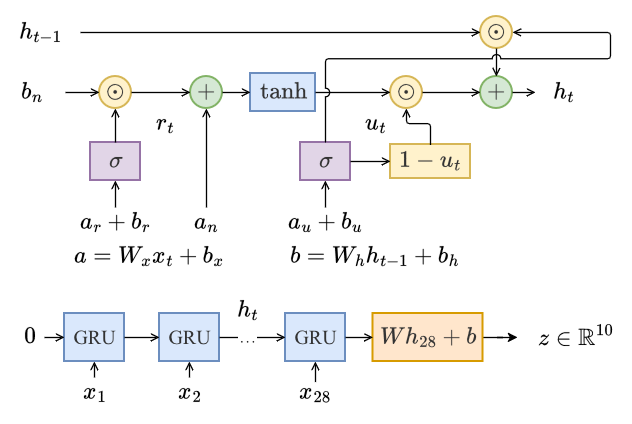
\includegraphics[width=0.95\linewidth]{Images/models/gru.png}
\caption{GRU cell and row-sequence classifier. The final hidden state feeds a linear classifier.}
\label{fig:model-gru}
\end{figure}

\subsubsection{Long short-term memory}
The LSTM has one layer with hidden size 128. It reads the same row sequence as
the GRU and applies a linear head to the final hidden state. It also maintains
a cell state $c_t$. Both states start at zero, and the updates follow the LSTM
equations in PyTorch documentation \cite{pytorch-lstm},
\begin{align*}
 q_t &= W_xx_t+b_x+W_hh_{t-1}+b_h,\\
 (i_t,f_t,g_t,o_t) &=
   \bigl(\sigma(q_{t,i}),\sigma(q_{t,f}),\tanh(q_{t,g}),\sigma(q_{t,o})\bigr),\\
 c_t &= f_t\odot c_{t-1}+i_t\odot g_t,\\
 h_t &= o_t\odot\tanh(c_t),
\end{align*}
where $q_t\in\mathbb{R}^{512}$ is divided into four 128-dimensional vectors.
The forget gate scales the existing cell state, the input gate controls the
candidate information added to it, and the output gate controls which part of
the updated cell state reaches the hidden state. This separates stored memory
from the state passed to the classifier, whereas the GRU uses one state for both.

\begin{figure}[htbp]
\centering
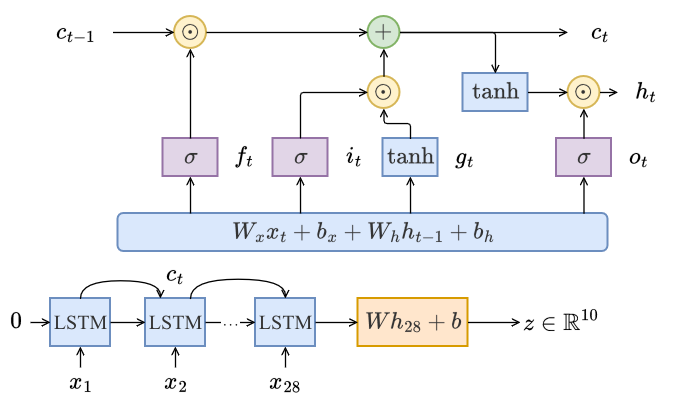
\includegraphics[width=0.95\linewidth]{Images/models/lstm.png}
\caption{LSTM cell and row-sequence classifier.}
\label{fig:model-lstm}
\end{figure}

\subsubsection{Transformer}
The Transformer uses the same row tokens as the recurrent models. Each token
is projected to 128 dimensions and receives a sinusoidal positional encoding.
Embedding dropout has probability $0.1$. Two encoder layers each apply
four-head self-attention and a feed-forward network of widths
$128\to2048\to128$, with ReLU. Each sublayer uses a residual connection
followed by layer normalization. Encoder dropout is $0.1$ \cite{pytorch-transformer}.

For a sequence representation $S\in\mathbb{R}^{H\times128}$, one attention
head computes
\begin{equation}
 Q=SW_Q,\quad K=SW_K,\quad V=SW_V,\qquad
 \operatorname{Attention}(Q,K,V)
 =\operatorname{softmax}\!\left(\frac{QK^\top}{\sqrt{32}}\right)V,
\end{equation}
where $W_Q,W_K,W_V\in\mathbb{R}^{128\times32}$ and the softmax acts across
key positions. Projection biases are omitted from this notation. The four
head outputs are concatenated and projected to 128 dimensions. The mean of
the encoded row vectors feeds a linear classifier. Attention connects
all row positions, while positional encoding supplies their order. Unlike the
recurrent models, attention relates rows directly rather than passing information
through every intervening row. Mean pooling then combines the encoded rows into
one vector for classification.

\begin{figure}[htbp]
\centering
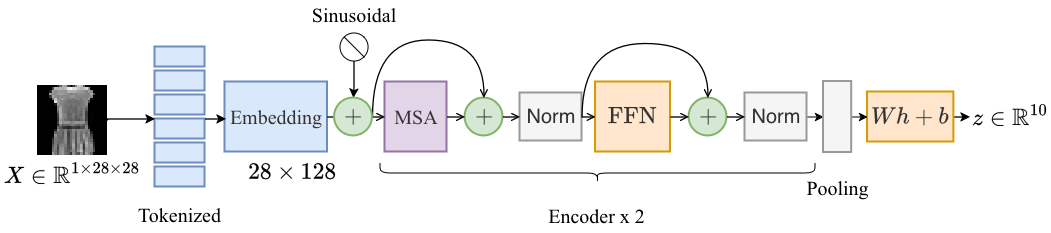
\includegraphics[width=0.95\linewidth]{Images/models/transformer.png}
\caption{Transformer with row embeddings, positional encoding, two encoder layers, and mean pooling.}
\label{fig:model-transformer}
\end{figure}

\subsection{Architecture comparison}
\label{sec:architecture-comparison}
\begin{table}[htbp]
\centering\small
\caption{Classifier dimensions and trainable parameters. MNIST and Fashion-MNIST share the same shapes.}
\label{tab:arch-comparison}
\begin{tabular}{lrrr}
\toprule
Model & Feature dimension $d$ & MNIST / Fashion-MNIST & CIFAR-10\\
\midrule
Linear & 784 / 3072 & 7,850 & 30,730\\
MLP & 128 & 235,146 & 820,874\\
CNN & 64 & 19,562 & 20,138\\
GRU & 128 & 61,962 & 88,074\\
LSTM & 128 & 82,186 & 117,002\\
Transformer & 128 & 1,191,050 & 1,199,754\\
\bottomrule
\end{tabular}
\end{table}

The models use the same epoch budget but differ in representation, size, and
regularization.

The group implements the model assembly, row-sequence processing, and GRU and
LSTM cell updates. Affine layers, convolution, normalization, pooling, and the
Transformer encoder use PyTorch modules \cite{pytorch-nn}.

\subsection{Loss and evaluation metrics}
\label{sec:metrics}

Let $\mathcal{D}=\{(x_i,y_i)\}_{i=1}^{N}$ denote a labelled sample, where
$y_i\in\{0,\ldots,K-1\}$ and $K=10$. For an input $x_i$, the model produces
a vector of logits $z_i=f_\theta(x_i)\in\mathbb{R}^{K}$. The corresponding
class probabilities and predicted label are
\begin{equation}
 p_{ik}=\frac{\exp(z_{ik})}{\sum_{j=0}^{K-1}\exp(z_{ij})},
 \qquad
 \hat y_i=\operatorname*{arg\,max}_{k}z_{ik}.
\end{equation}

\paragraph{Training objective.}
All models minimize the mean categorical cross-entropy,
\begin{equation}
 \mathcal{L}_{\mathrm{CE}}(\theta;\mathcal{D})
 =-\frac{1}{N}\sum_{i=1}^{N}\log p_{i,y_i}
 =\frac{1}{N}\sum_{i=1}^{N}
 \left[\log\sum_{k=0}^{K-1}\exp(z_{ik})-z_{i,y_i}\right].
\end{equation}
We compute cross-entropy directly from logits without applying softmax first.
Each optimization step uses the mean loss of its minibatch. Cross-entropy
penalizes a low probability for the true class, so two predictions with the same
argmax can contribute different losses. Validation loss therefore considers
confidence in addition to whether the predicted label is correct.

\paragraph{Classification performance.}
Define the confusion matrix $C$ by
\begin{equation}
 C_{ab}=\sum_{i=1}^{N}\mathbf{1}\{y_i=a,\ \hat y_i=b\},
\end{equation}
where rows correspond to true classes and columns to predicted classes.
Accuracy is the proportion of correct predictions,
\begin{equation}
 \mathrm{Accuracy}=\frac{1}{N}\sum_{k=0}^{K-1}C_{kk}.
\end{equation}

For class $k$, let
$\mathrm{TP}_k=C_{kk}$,
$\mathrm{FP}_k=\sum_{a\ne k}C_{ak}$, and
$\mathrm{FN}_k=\sum_{b\ne k}C_{kb}$.
We report the unweighted mean of the class F1 scores,
\begin{equation}
 F_{1,k}=\frac{2\mathrm{TP}_k}
 {2\mathrm{TP}_k+\mathrm{FP}_k+\mathrm{FN}_k},
 \qquad
 \mathrm{Macro\text{-}F1}=\frac{1}{K}\sum_{k=0}^{K-1}F_{1,k}.
\end{equation}
Macro-F1 gives each class equal weight. We compute both metrics over the full
evaluation split. Accuracy measures how often the predicted label is correct,
while macro-F1 combines precision and recall for each class before averaging.
Since Fashion-MNIST is balanced, differences between these metrics reflect the
pattern of class errors rather than unequal numbers of test images.

\paragraph{Class-level analysis.}
Per-class recall measures the fraction of examples of a true class that the
model identifies correctly,
\begin{equation}
 R_k=\frac{C_{kk}}{\sum_b C_{kb}}.
\end{equation}
We normalize each row as $\widetilde C_{ab}=C_{ab}/\sum_j C_{aj}$.
The diagonal gives class recall. Off-diagonal values show the fraction of each
true class assigned to an incorrect class.

\paragraph{Model size and computation.}
We count trainable parameters in the encoder and classification head, excluding
buffers and optimizer state. Parameter count measures storage for model weights,
not the operations needed for a prediction.

\subsection{Training configuration}
\label{sec:training-setup}
\begin{table}[htbp]
\centering\small
\caption{Training settings for the reported runs.}
\label{tab:training-setup}
\begin{tabular}{ll}
\toprule
Setting & Value\\
\midrule
Optimizer & Adam, $\beta_1=0.9$, $\beta_2=0.999$, $\epsilon=10^{-8}$\\
Learning rate & $10^{-3}$, constant\\
Batch size & 128\\
Epochs / seed & 50 / 42\\
Validation fraction & 0.1 of the official training split\\
Weight decay & 0\\
Arithmetic & Float32, no mixed precision\\
Checkpoint rule & Minimum validation cross-entropy\\
MLP dropout & 0.2 after each hidden activation\\
Transformer dropout & 0.1 in embeddings and encoder layers\\
CNN normalization & Batch normalization after each convolution\\
\bottomrule
\end{tabular}
\end{table}

All models use the preprocessing and augmentation in
Section~\ref{sec:preprocessing}. CNN evaluation uses an NVIDIA GeForce RTX 4060 Ti
with Python 3.11.11 and PyTorch 2.14.0+cu126. Other runs use macOS ARM and CUDA
environments.

\subsection{Comparison protocol}
\label{sec:experiment-design}
We compare Linear, MLP, CNN, GRU, LSTM, and Transformer on Fashion-MNIST.
Within each dataset, all models share the split, preprocessing, augmentation,
optimizer settings, epoch budget, and checkpoint rule. This compares the models
under one common training recipe. It does not give each architecture a separately
tuned optimizer or schedule, so the ranking applies to this recipe rather than
the best result each architecture could achieve.

For the detailed comparison with CNN, we choose the flattened-pixel baseline
with the lower minimum validation loss among Linear and MLP. A tie favours
Linear. This selects MLP. Both models are evaluated on the same official test
images. Confusion matrices and class recall use all test predictions.
For the qualitative comparison, we show the first two test images in each of
three categories: CNN correct and MLP wrong, both wrong, and MLP correct and CNN
wrong. We count the full test set separately to measure how often each outcome
occurs.
